\chapter{Introduction}
\label{ch:intro}
The absence of risks in software is essential and highlights what ensures that the software will perform as expected and not cause unintended consequences. Unfortunately, that feautere is not present most time.\\\\
For critical systems, such as those used in the medical or aerospace industries, the stakes are even higher. These systems must be thoroughly tested and validated to ensure that they will not cause harm or failure in a critical situation. For example:
\begin{itemize}
	\item Medical systems: Medical systems such as electronic health records (EHRs) and medical devices are critical systems that can have serious consequences if they fail. A bug in an EHR system could lead to incorrect patient information being displayed, potentially leading to a misdiagnosis or other medical errors.
	\item Aerospace systems: Aerospace systems such as aircraft navigation systems and flight control systems are critical systems that must operate reliably at all times. A bug in an aircraft navigation system could cause the plane to fly off course, leading to a crash.
	\item Industrial control systems: Industrial control systems (ICS) are used to control and monitor industrial processes such as manufacturing, power generation, and oil and gas production. An issue in an ICS could cause a malfunction in a manufacturing process, leading to costly downtime or even physical damage to the equipment, or even a cyber-attack on an ICS could cause a shutdown of the whole process causing a major disruption.
\end{itemize}
The most used way to guarantee software quality and detect errors is testing, so it is essential to perform it in the best possible way.\\
\begin{align*}
	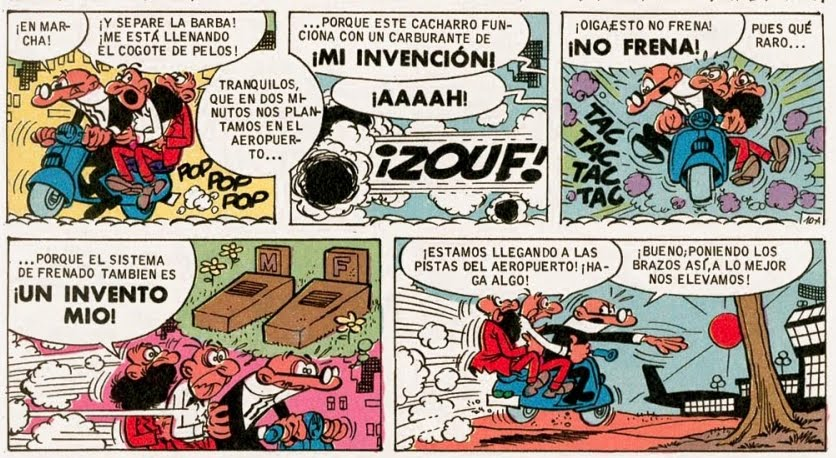
\includegraphics[scale=0.4]{vineta-mortadelo-filemon}
\end{align*}
%
\section{Testing}
%
Software testing (or simply testing) is the process of evaluating a system or its component(s) to find whether it satisfies the specified requirements. It consists of executing a program on a known pre-selected set (test suite) of inputs (test cases) and inspecting whether the outputs match the expected results.\\\\
This process validates the semantic properties of a program's behaviour \cite{pbtnewapproach}. It's important to test software thoroughly before deployment to ensure it functions as intended and to identify and fix bugs or other issues. Testing is an essential step in the software development process and is critical for ensuring the quality and reliability of software.\\\\
Therefore, we can define in a relaxed way that a \textbf{test} is a set of executions on a given program using different input data for each execution; its purpose is to determine if the program functions correctly. A test has a negative result if an error is detected during the test i.e., the program crashes or a property is violated. \cite{pbtnewapproach} \cite{arttesting} \\

A test has a positive result if a series of tests produces no error, and the series of tests is "complete" under some coverage metric. When we say in software testing that a test is "complete", it refers to the level of coverage the tests provide for the software being tested. In other words, that reflects a representative percentage of the reliability of the software with respect to expected behaviour. However, we have to consider that "reliability" is relative and it is biased and subject to the chosen test cases, which is itself subject to the criteria of the tester \cite{arttesting}. \\

A test has an "incomplete" result if a series of tests produces no errors but the series is not complete under the coverage metric. In summary, a test is focused on evaluating the software to find any issues and bugs \cite{pbtnewapproach}.\\\\
There are different types of tests that can be used during the software development process, each with a different purpose and focus. Some of the main types of tests are:
%%
\begin{itemize}
	\item \textbf{Unit testing}: Unit testing is a type of testing that focuses on individual components of the software, such as individual functions or methods. Unit testing aims to ensure that each component behaves as expected. Unit tests are usually automated, and they are run as part of the development process to catch any issues early.
	\item \textbf{Integration testing}: Integration testing is used to ensure that different software components work together correctly. It tests the interactions between different parts of the software. Integration tests are usually automated, and they are run after the unit tests to ensure that the integrated system behaves as expected.
	\item \textbf{Acceptance testing}: Acceptance testing is used to ensure that the software meets the needs of the end users. It is typically done by the customer or other stakeholders to ensure that the software meets their needs. Acceptance tests can be automated or manual, and they are run after system tests to ensure that the system is ready to be deployed.
\end{itemize}
%%
Sadly, trying to find counter-examples by testing that produces bugs a behaviour non-expected is most of the time a difficult task. In simpler software, testers could find most of those cases which produce counter-examples, designing test cases one by one. However, the design process reaches those cases that one knows by experience or intuition, leaving aside very interesting and not at all intuitive cases that can hardly be imagined \cite{pbtnewapproach} \cite{arttesting}. For this reason and because it can be a very tedious task, it would be ideal to automate the generation of test cases.

\subsubsection*{Testing and Specificaions}
%% Revisar
Also, during the life-cycle of software development has used several known techniques in order to get free-bugs software in an efficient and proper way. The most common paradigm, which is also the most natural way, is test driven development (a.k.a TDD) \cite{tddpaper}. \\

TDD is a software development technique in which tests are developed before the code, in short and incremental cycles. This technique proposes for the developer to create a new flawed test, and then to implement a little piece of code, in order to satisfy the current test set \cite{efftdd}. Then, the code is refactored if necessary, to provide a better structure and architecture for the current solution. \\\\
%%
The challenge addressed in this work is to use TDD in applications with non-deterministic behaviour as stated before. Although it is not possible to know exactly what the output will be, it is usually possible to check whether the generated output is valid or not \cite{arttesting}. \\\\
%%
The following factors make it difficult to develop randomized software using TDD \cite{tddpaper}: 
\begin{itemize}
	\item Results for each execution may be different for the same inputs, which makes it difficult to validate the return value.
	\item Obtaining a valid return for a test case execution does not mean that valid return will be delivered on the next executions.
	\item The random decisions and their paths number make it not viable to create Mock Objects that return fixed results for these decisions.
	\item It is difficult to execute a previous failed test with the same random decisions undertaken in its former execution.
\end{itemize}
%%
In conclusion, you have to iterate several times in case of testing fails. \\\\
%%
On the other hand, some techniques like correctness by constructions, try to formalize some specifications and build code based on them \cite{correctnesspaper}.\\\\
%%
The idea is to start with a succinct specification of the problem, which is progressively evolved into code in small, tractable refinement steps. Experience has shown that the resulting algorithms are invariably simpler and more efficient than solutions that have been hacked into correctness. Furthermore, such solutions are guaranteed to be correct (i.e. they are guaranteed to comply with their specifications) in the same sense that the proof of a mathematical theorem is guaranteed to be correct. Here you don't have to iterate too as other ones, but the formalized process is, in general, a complex task.\\\\
%%
For many reasons, in order to get a good enough solution for testing, property-based testing was coming up.

\section{Property-Based Testing}

Property-based testing (a.k.a PBT) is a technique that uses inputs generated by specifications to test the properties of a system, rather than specific or random inputs. It helps to mitigate risks in the software industry by providing an automated way to test the software in a wide range of scenarios using randomly generated test cases. This can help to identify bugs and other issues that may not be found using traditional testing techniques such as manual testing or unit testing \cite{pbtfree}.\\\\
%%
The use of randomly generated inputs in PBT allows for a more thorough exploration of the software's behaviour, making it more likely that any bugs or issues will be found. It also helps to ensure that the software behaves correctly in a wide range of scenarios, which is especially important for critical systems.\\\\
%%
PBT helps to ensure that the software is robust and can handle unexpected inputs or edge cases. This is particularly important for systems where failure could have serious consequences. Also helps in testing the software performance and scalability, by testing the software with large inputs, it can identify potential performance issues that would be difficult to detect with other testing techniques.\\\\
%% Revisar desde aqui
The specification of one or more properties is the driver of the testing process, which assures that the given program meets the stated property, leaving aside the task of generating valid inputs \cite{pbtnewapproach}.\\\\
%%
For example, if an analyst wants to validate that a specific program correctly authenticates a user, a property-basted testing procedure tests the implementation of the authentication mechanisms in the source code to determine if the code meets the specification of \textit{correctly authenticating the user}.\\\\
%%
Specifications state what a system should or should not do. The advantage of using specifications is the formalism they establish for verifying proper (or improper) program behaviour. PBT validates that the final product is free of specific flaws. Because PBT concentrates on generic flaws, it is ideal for focusing on analysis late in the development cycle after program functionality has been established \cite{strtyped}.\\\\
%% Usar esto para la solución
In a property-based framework, test cases are automatically generated and run from assertions about the logical properties of the program. Feedback is given to the user about their evaluation \cite{pbtnewapproach} \cite{pbtfree}.\\\\
PBT naturally is based on the logic programming paradigm. Assertions are first-order formulas and thus easily encoded as program predicates. Therefore, a property-based approach to testing is intuitive for the logic programmer.

\section{Problem: Test cases that satisfy a given specification}

Property-Based testing provides a helpful solution to generate random test cases for testing. And it is good enough for most pieces of code that want to test. However, we will put focus on those functions that assume inputs with preconditions. \cite{pbtfree}\\
\begin{example}[Sorted Lists]
	Let $S$ be a set, $\mathtt{xs}$ a list of elements of $S$, and consider the ordering relationship $\preceq$ over elements of $S$. We can say that $xs$ is an \textbf{ordered list} if it holds one of the following invariants:
	%%
	\begin{description}
		\item[\tav \tav$\mathtt{INV1}$] $xs$ is empty.
		\item[\tav \tav$\mathtt{INV2}$] $\forall xss$ sublist of $xs$ with $xss \neq \emptyset$, $\exists a \in xss$ such that $\forall x \in xss, a \preceq x$ holds.
	\end{description}
	%%
	Let's suppose we want to test the behaviour of our \texttt{insertOrdered} function which its expected behaviour should be the following:\\\\
	%%
	$\mathtt{PROP1}$ \textit{Given an ordered list,} \texttt{insertOrdered} \textit{inserts an element and its result is an ordered list}.\\
	%%
	\lstinputlisting[language=Haskell, label=samplecode, caption=Insert an element in an ordered list]{sections/code/example/insertOrdered.hs}
	%%
	\lstinputlisting[language=Scala, label=samplecode, caption=Insert an element in an ordered list (Scala version)]{sections/code/example/insertOrdered.scala}
	%%
	A property-based testing framework should generate several enough random \textbf{ordered lists} to check if $\mathtt{PROP1}$ holds. This is not as easy as you could think. Let's do our own mental exercise step by step. Let's suppose we have a good PBT framework:
	\begin{enumerate}
		\item First of all, the framework has to generate randomly a set of lists.
		\item Then, it has to check which one of them is an \textbf{ordered list}, i.e, it has to check if holds either $\mathtt{INV1}$ or $\mathtt{INV2}$.
		\item Finally checks if the property $\mathtt{PROP1}$ holds, which means the result has to be an \textbf{ordered list}, i.e. it has to check if holds either $\mathtt{INV1}$ or $\mathtt{INV2}$ too.
	\end{enumerate}
	This process is more complex, but for this moment we can consider this friendly description. We will deeply get ahead in the following chapters.\\\\
	%%
	Therefore, imagine that your PBT framework generates $100$ randomly generated lists in every iteration. Probably, one or, if you have lucky, two lists of them are ordered lists.\\\\
	%%
	On the one hand, it is so difficult to achieve so many scenarios (at least in a shorter time). Also, the framework probably brings you just the same empty list (because it is the easiest generated test case that holds one of the invariants) as the input value for checking the property which would make the results unreliable.\\\\
	%%
	And on the other hand, the property $\mathtt{PROP1}$ is relatively simple but, what happens if we consider a more complex property? For example, we can consider a red-black tree.\\
\end{example}
%%
\begin{example}[Red-Black Tree]
	A \textbf{red-black tree} is a binary search tree where each node has two labels: a color $\mathtt{C}$, which is either $\mathtt{red}$ ($\mathtt{R}$) or $\mathtt{black}$ ($\mathtt{B}$), and an integer $\mathtt{N}$. For the purpose of test generation, node values are abstracted away in the definition of the data structure:
	\begin{equation*}
		\begin{array}{rll}
			\mathtt{C}    & ::= & \mathtt{R} \texttt{ | } \mathtt{B}                        \\
			\mathtt{N}    & ::= & \ldots \texttt{ | -1 | 0 | 1 | } \ldots                   \\
			\mathtt{Tree} & ::= & \mathtt{nil} \texttt{ | } \mathtt{C \; N \; Tree \; Tree} 
		\end{array}
	\end{equation*}
	A red-black tree must also satisfy the following three invariants:
	%%
	\begin{itemize}
		\item[\tav \tav$\mathtt{INV1}$] Every path from the root to a leaf has the same number of black nodes
		\item[\tav \tav$\mathtt{INV2}$] No red node has a red child and
		\item[\tav \tav$\mathtt{INV3}$] For every node $n$, all the nodes in the left (respectively, right) subtree of $n$, if any, have keys that are smaller (respectively, bigger) than the key labeling $n$.
	\end{itemize}
	%%
	Since red-black trees enjoy a weak form of balancing, operations such as inserting, deleting, and finding values are more efficient, in the worst case, than in ordinary binary search trees.\\\\
	%%
	Let's suppose we want to test the behaviour of our \texttt{insertOrderedRBTree} function which its expected behaviour should be the following:\\\\
	%%
	$\mathtt{PROP2}$ \textit{Given a red-black tree,} \texttt{insertOrderedRBTree} \textit{inserts an element and its result is a new tree which is a red-black tree}. \\\\
	%%
	The following code is inspired by the Haskell ADT definition of red-black trees in \cite{rbtreehaskell}.
	%%
	\lstinputlisting[language=Haskell, label=samplecode, caption=Definition of red-black tree ADT]{sections/code/example/rbtree.hs}
	%%
	\lstinputlisting[language=Haskell, label=samplecode, caption=Insert an element in an red-black tree]{sections/code/example/insertOrderedRBTree.hs}
	%%
	\lstinputlisting[language=Scala, label=samplecode, caption=Definition of red-black tree ADT (Scala version)]{sections/code/example/rbtree.scala}
	%%
	\lstinputlisting[language=Scala, label=samplecode, caption=Insert an element in an red-black tree (Scala version)]{sections/code/example/insertOrderedRBTree.scala}
	%%
\end{example}
%%
Following the same reasoning that we did before, the reader can deduce how complex is the task.\\\\
%%
In general, PBT is not prepared to generate inputs with preconditions, let alone input with complex ones.

\section{Our Approach}

Building \textit{generators} to create test cases that property-based testing use to test software behaviour is a hard, quite costly, and error-prone task. Even though most property-based testing frameworks cover simple scenarios, there are many troubles with preconditioned generated test cases as we have just seen.\\\\
%%
In contrast to the recent works \cite{genclp} \cite{effgenttransf}, what we propose is (1) to build an efficient and automatic generator of input test values that satisfy a given specification and (2) provide a language syntax-driven bijection between the origin language's expressions and the constraint logic programming language ones which can translate and map expression from one language to other. In particular, we will consider the case when the input values are algebraic data types satisfying complex constraints. The generation process is performed via symbolic execution in the CLP language of the translated expressions of those ADTs and their specifications.\\\\
%%
We will focus on the \textbf{strong and static well-typed} language Haskell and we will use Prolog as CLP language. Although it is well known that the mainly property-based testing framework for Haskell is \textbf{QuickCheck}, and it has its own \textit{generators}, we will provide steps to build a mechanism to generate those kinds of preconditioned input values. In particular, we will explore how to create a model that maps Haskell's ADT expressions and its specification to Prolog expression, generate symbolic Prolog expressions that hold the specifications and returns those expressions to Haskell. \\\\
%%
Following the recent state-of-the-art approach, we use a \textit{declarative} language such as Haskell following those works that are based on using CLP languages as generators. Being a declarative language allows us to separate the process of defining the algebra data type structure expression and their constraints from their semantics or instances. This separation helps improve the correctness of the developed test case generators, which implies that we can separate between \textit{what} we want to generate in an expressive way \cite{genclp}.\\\\
%%
But the main reason is the nature of being static-typed. It allows us to reason about types in a safe way and also we gain in static type checking in compile time, which adds us a plus about program verification. Therefore, Haskell allows to support us the fact that algebraic data types expressions are their own type (the 'ADT' type that corresponds), and then, intuitively and implicitly, we can assume and reason the ADT's invariants holds thanks to the fact that they are from that type (the 'ADT' type).\\\\
%%
In contrast to the recent works \cite{smtbased} that use Z3 or some SMT solver such as a test generator and output test validator. We use constraint logic programming language such as our test generator.\\\\
%%
This approach fits better with our purpose thanks to how flexible, expressive, and descriptive the syntax of both languages Haskell and Prolog are. In fact, we show how natural is to define an algebraic data type in Haskell and find an expression 'equivalent' (in the sense of translation) in Prolog. This leads us to find a mechanism that translates both languages' expressions which also can fit so well with the Erlang language.\\\\
%%
However, in contrast to the recent state-of-the-art research and regarding to the mentioned Erlang language, we use \textbf{static-typed and strong-typed} language.\\\\
%%
The use of dynamic language could provocate non-safety in its type checking, and therefore, we cannot ensure what type is working when we deal with a given formal expression. For instance, in Erlang we can have both $\texttt{adt}:\tau_1$ and $\texttt{adt}:\tau_2$, which their formal expression is $\texttt{adt}$. When we generate test cases for that expression and come back to Erlang, we could provide wrong test input values \cite{strtyped} \cite{stvsdt}. \\\\
%%
There seems to be some controversy about the advantages of static vs dynamic typing \cite{stvsdt} \cite{strtyped}. Type-checking provides another barrier against nonsensical programs. Moreover, whereas in a dynamically typed language,   type mismatches would be discovered at runtime, in strongly typed statically checked languages type mismatches are discovered at compile time, eliminating lots of incorrect programs before they have a chance to run \cite{strtyped}.
%%
\begin{displayquote}
	Languages without type systems or even safe, dynamically checked languages, tend to offer features or encourage programming idioms that make type-checking difficult or infeasible. \\ ... \\
	The assertion that types should be an integral part of a programming language is separate from the question of where the programmer must physically write down type annotations and where they can instead be inferred by the compiler. A well-designed statically typed language will never require huge amounts of type information to be explicitly and tediously maintained by the programmer. \cite{cpierce}
\end{displayquote}
%%
In Haskell, the definition of the ADT expression is itself the declaration of the type to which it belongs. That means, we cannot type two ADT with the same expression and try belonging on different types. There is a univocal relationship between the ADT's expression and the its type. \\\\
%%
Finally, for the purpose of this work, we will illustrate all these concepts and ideas by applying them while writing a generator for red-black trees. As we defined before:\\
%%
\begin{definition*}[Red-Black Tree]
	A \textbf{red-black tree} is a binary search tree where each node has two labels: a color $\mathtt{C}$, which is either $\mathtt{red}$ ($\mathtt{R}$) or $\mathtt{black}$ ($\mathtt{B}$), and an integer $\mathtt{N}$. For the purpose of test generation, node values are abstracted away in the definition of the data structure:
	\begin{equation*}
		\begin{array}{rll}
			\mathtt{C}    & ::= & \mathtt{R} \texttt{ | } \mathtt{B}                        \\
			\mathtt{N}    & ::= & \ldots \texttt{ | -1 | 0 | 1 | } \ldots                   \\
			\mathtt{Tree} & ::= & \mathtt{nil} \texttt{ | } \mathtt{C \; N \; Tree \; Tree} 
		\end{array}
	\end{equation*}
	A red-black tree must also satisfy the following three invariants:
	%%
	\begin{description}
		\item[\tav \tav$\mathtt{INV1}$] Every path from the root to a leaf has the same number of black nodes
		\item[\tav \tav$\mathtt{INV2}$] No red node has a red child and
		\item[\tav \tav$\mathtt{INV3}$] For every node $n$, all the nodes in the left (respectively, right) subtree of $n$, if
		any, have keys that are smaller (respectively, bigger) than the key labeling $n$.
	\end{description}
\end{definition*}
%%
The definition of this structure, which holds a set of complex invariants, can be defined as an algebraic data type in Haskell as follow:
%%
\lstinputlisting[language=Haskell, label=samplecode, caption=Definition of red-black tree ADT]{sections/code/example/rbtree.hs}
%%
We can deduce that the expression \texttt{Nil} and \texttt{T Color a (Tree a) (Tree a)} in Haskell can be mapped to the expressions \texttt{nil} and \texttt{t(C,X,L,R)} in Prolog, respectively; where \texttt{C} is the color (either \texttt{red} or \texttt{black}), and both \texttt{L}, \texttt{R} are red-black trees too, i.e., they can be expressed as \texttt{nil} or \texttt{t(C',X',L',R')}. This brings us light on our hard way, don't you?. Let's see an example before starting this work.\\
\begin{definition*}[Sorted Lists]
	Let $S$ be a set, $\mathtt{xs}$ a list of elements of $S$, and consider the ordering relationship $\preceq$ over elements of $S$. We can say that $xs$ is an \textbf{ordered list} if it holds one of the following invariants:
	%%
	\begin{description}
		\item[\tav \tav$\mathtt{INV1}$] $xs$ is empty.
		\item[\tav \tav$\mathtt{INV2}$] $\forall xss$ sublist of $xs$ with $xss \neq \emptyset$, $\exists a \in xss$ such that $\forall x \in xss, a \preceq x$ holds.
	\end{description}
	First of all, we have to identify the Haskell lists' syntax expression, that is:
\end{definition*}
%%
A list expression in Haskell could be either $\texttt{[]}$ or $\texttt{x:xs}$ syntax.
Therefore, the list ADT could be expressed in Prolog as follows $\texttt{[]}$ or $\texttt{X:Xs}$, respectively.\\\\
%%
Then, in order to provide the invariants $\mathtt{INV1}$ and $\mathtt{INV2}$ and get a definition of a sorted list in Prolog, we should translate in someway these two (written in Haskell or, more precisely written in Liquid Haskell) or type directly in scratch the restrictions in Prolog to get the following expressions or similar:
%%
\begin{description}
	\item[\tav \tav$\mathtt{INV1}$] $\texttt{sorted\_list([])}$ which holds that an empty list is a sorted list.
	\item[\tav \tav$\mathtt{INV2}$] $\texttt{sorted\_list(\_:[])}$ which holds that a one-element list is a sorted list.
	\item[\tav \tav$\mathtt{INV2}$] $\texttt{sorted\_list(X1:X2:Xs) :- X1 \#=< X2, sorted\_list(X2:Xs)}$ which means that a list is a sorted list if it holds that every two elements hold an ordering relationship and the tail of the list is a sorted list too.
\end{description}
%%
In resume, we should map the Haskell definition of a sorter list to some Prolog definition like this:
%%
\lstinputlisting[language=Prolog, label=sortedlistprolog, caption=Sorted List in Prolog]{sections/code/example/haskell_sorted_list.pl}

With this implementation, we can get the following test cases using, for instance, the Prolog-CLI prompt and the expression $\texttt{sorted\_list}$.
%%
%% Insertar imagen del prompt
%%
However, readers can think that modeling list adt and the invariants for sorted list could be a little bit easy. Let's see a final challenge that shows interest in this approach.\\
%% Preguntar a Julio sobre una definicion más formal
\begin{definition*}[Binary Search Tree]
	A binary search tree (BST) is a tree in which all the nodes follow the below-mentioned properties.
	\begin{itemize}
		\item The left sub-tree of a node has a key less than or equal to its parent node's key.
		\item The right sub-tree of a node has a key greater than or equal to its parent node's key.
	\end{itemize}
	A binary search tree must also satisfy the following invariants:
	\begin{description}
		\item[\tav \tav$\mathtt{INV1}$] An empty tree is a binary search tree.
		\item[\tav \tav$\mathtt{INV2.1}$] The left sub-tree is a binary search tree.
		\item[\tav \tav$\mathtt{INV2.2}$] The right sub-tree is a binary search tree.
	\end{description}
\end{definition*}
Here we can see that invariants not only are more complex than the sorted list example but also it holds recursively onto their inner structures. Therefore, getting a test case for this example is a hard task. But we can do as before. First of all, we have to identify the Haskell \ttt{bst}' syntax expression, that is:\\\\
%%
A \ttt{bst} expression in Haskell could be either $\texttt{Nil}$ or $\texttt{T a BSTree a BSTree a}$ syntax.
Therefore, the \ttt{bst} ADT could be expressed in Prolog as follows $\texttt{nil}$ or $\texttt{t(N,L,R)}$.\\\\
%%
Then, in order to provide the invariants $\mathtt{INV1}$, $\mathtt{INV2.1}$ and $\mathtt{INV2.2}$ and get a definition of a \ttt{bst} in Prolog, we do as similar as before to get the following expressions or similar:
%%
\begin{description}
	\item[\tav \tav$\mathtt{INV1}$] $\texttt{bst(nil)}$ which holds that an empty tree is a binary search tree.
	\item[\tav \tav$\mathtt{INV2.1}$ and $\mathtt{INV2.2}$] $\texttt{bst(t(\_,nil,nil))}$ defines a non-empty tree with no left or right subtrees, which holds that a one-element tree is a binary search tree.
	\item[\tav \tav$\mathtt{INV2.1}$] $\texttt{bst(t(N,L,nil)) :- L = t(LN,\_,\_), LN \#< N, bst(L)}$ defines a non-empty tree with a left subtree and no right subtree.
	\item[\tav \tav$\mathtt{INV2.2}$] $\texttt{bst(t(N,nil,R)) :- R = t(RN,\_,\_), RN \#> N, bst(R)}$ defines a non-empty tree with a right subtree and no left subtree.
	\item[\tav \tav$\mathtt{INV2.1}$ and $\mathtt{INV2.2}$]
	\begin{flalign*}
		\texttt{bst(t(N,L,R))} \texttt{:-} & \texttt{L = t(LN,\_,\_), LN \#< N, bst(L)} && \\
		& \texttt{R = t(RN,\_,\_), RN \#> N, bst(R)} &&
	\end{flalign*}
	defines a non-empty tree with both left and right subtrees.
\end{description}
%%
In resume, we should map the following Haskell definition of a binary search tree:
%
\lstinputlisting[language=Haskell, label=bstreehaskell, caption=binary search tree in Haskell]{sections/code/example/bst.hs}
%
to some Prolog definitions like this:
%%
\lstinputlisting[language=Prolog, label=sortedlistprolog, caption=Sorted List in Prolog]{sections/code/example/bst.pl}
%
\section{Related Works}

\subsection{QuickCheck: Automatic testing of Haskell programs}

\bhref{https://hackage.haskell.org/package/QuickCheck}{QuickCheck} \cite{quickcheck} is a library for random testing of program properties. The programmer provides a specification of the program, in the form of properties that functions should satisfy, and QuickCheck then tests that the properties hold in a large number of randomly generated cases. Specifications are expressed in Haskell, using combinators provided by QuickCheck. QuickCheck provides combinators to define properties, observe the distribution of test data, and define test data generators. \\\\
%%
QuickCheck is one of the original property-based testing frameworks. It was developed in 1999 as a tool for Haskell, and it has since been ported to other languages such as Erlang, Scala, and Clojure. QuickCheck uses random input generation and shrinking to automatically generate test cases for a given property.
\cite{qcrepo}

\subsection{ScalaCheck: Automatic testing of Scala and Java programs}

\bhref{https://scalacheck.org/index.html}{ScalaCheck} is a library written in Scala and used for automated property-based testing of Scala or Java programs. ScalaCheck was originally inspired by the Haskell library QuickCheck but has also ventured into its own. ScalaCheck is used by several prominent Scala projects, for example, the \bhref{https://www.scala-lang.org/}{Scala compiler} and the \bhref{https://akka.io/}{Akka} concurrency framework. \cite{screpo}

\subsection{PropEr: Property-based testing tool for Erlang}

\bhref{https://proper-testing.github.io/}{PropEr} is a QuickCheck-inspired open-source property-based testing tool for Erlang, developed by Manolis Papadakis, Eirini Arvaniti, and Kostis Sagonas.\\\\
%%
PropEr is a property-based testing tool, designed to test programs written in the Erlang programming language. Its focus is on testing the behaviour of pure functions. On top of that, it is equipped with two library modules that can be used for testing stateful code. The input domain of functions is specified through the use of a type system, modeled closely after the type system of the language itself. Properties are written using Erlang expressions, with the help of a few predefined macros. \cite{pprepo}

\subsection{Hypothesis: Property-based testing tool for Python}

\bhref{https://hypothesis.readthedocs.io/en/latest/}{Hypothesis} is a modern property-based testing library for Python. It's similar to the previously mentioned frameworks but with some differences, it also provides features like stateful testing and advanced strategies for input generation. \cite{hprepo}

\section{Test Cases with Pre-Condition(s)}

Efforts to provide best-fitted generators to complex constrained test cases are becoming a very current research topic. It is faced from some perspectives.\\\\
%%
Regarding to Fioravanti et al. research works \cite{pbtfree}, \cite{genclp} and \cite{effgenttransf}, we can observe a long projection to provide a similar approach. Indeed, in \cite{pbtfree} and \cite{genclp}, they are based on the idea to relieve the developer from the task of writing data generators of valid inputs using CLP languages. They show how using CLP languages for that propose and prove how many benefits and how efficient is to use these kinds of logic programming languages as test generators.\\\\
%%
Finally, in \cite{effgenttransf}, they bring us some kinds of best-performances using program transformation instead of the classical and native left-to-right strategy implemented by standard CLP systems which can very inefficient. These works, in essence, propose a framework based on Constraint Logic Programming for the systematic development of generators of large sets of structurally complex test data structures.\\\\
%%
They adopt a declarative approach too following the so-called \textit{constrain-and-generate} approach. However, they focus on the \textbf{dynamically typed} functional programming language Erlang and refer to how arduous the task of writing a generator that satisfies all constraints defined by a filter for the PropEr framework is.\\\\
%%
Ricardo Peña et al. research works in \cite{smtbased} propose a system that can automatically generate an exhaustive set of black box test cases, up to a given size, for programs under test requiring complex preconditions. The key of this research is how they translate a formal precondition into a set of constraints belonging to the decidable logic of SMT solvers. They use an \textbf{SMT solver as a test case generator} to directly generate test cases satisfying a complex precondition. Also, they describe both black-box and white-box approaches to fit searching strategies for those test cases.
%%
\section{Thesis Organization}
We will discuss the organization of the content and provide a brief overview of the different topics that will be covered throughout the book. We will focus on two main aspects: Haskell and Prolog.
%%
\begin{enumerate}
	\item In this preliminary chapter 2, we will explore the basic concepts of Haskell and Prolog. We will discuss the roles these languages play in the context of the thesis and analyze their formal syntax.
	\begin{itemize}
		\item Haskell: We will explain what Haskell is and its significance in functional programming. We will discuss its key features and how it relates to the translation approach that will be employed later on.
		\item Haskell Syntax: We will analyze the specific syntax of Haskell that facilitates the translation of expressions. We will discuss the constructions and conventions used to represent. 
		\item Prolog: We will introduce Prolog, a logic programming language. We will describe its utility and how it applies to problem-solving based on logical rules. We will analyze its formal syntax and highlight relevant aspects for translating algebraic data type expressions to Prolog expressions such that recursive definitions.
		\item Prolog Syntax: We will explore the Prolog syntax necessary for receiving and processing the translated expressions from Haskell. We will discuss how logical rules are structured in Prolog and how they can be used to manipulate and evaluate the expressions sent from Haskell.
	\end{itemize}
	\item In chapter 3, we will present a translation mechanism guided by Haskell syntax to send algebraic data types expressions to Prolog expressions. We will provide the necessary foundations to understand and utilize the translation mechanism from Algebra data types to Prolog expressions, laying the groundwork for subsequent chapters that delve deeper into these concepts and present practical applications.
\end{enumerate}